\documentclass[a4paper]{article}

\usepackage{fullpage}
\usepackage{amsmath}
\usepackage{graphicx}
\usepackage[bottom]{footmisc}
\usepackage{hyperref}
\usepackage{syntax}


\newcommand{\heart}{\ensuremath\heartsuit}

%\usepackage[latin1]{inputenc}
%\usepackage[T1]{fontenc}
%\usepackage{ngerman} 
\title{Functional Languages}
\author{Project - Turtle Graphics II}

\date{02.12.2019}

\begin{document}

\maketitle

\section{More turtle graphics}

This part of the project is based on the previous one. You can either extend your current solution or you can start off with our provided template\footnote{\url{https://github.com/erdferkel-teaching/turtleWS19/tree/PartTwoSkeleton}}.
In order to reduce programming efforts you don't need to adapt your parser. In this exercise it is sufficient to extend the interpreter and the domain model.
In case you extend your current solution, you need to adapt the main entry point in the graphics code in order to support animation (as demonstrated
in the provided template). We measure the current time of a rendered frame and pass it to the update function as animation timestamp\footnote{Thus, if you use the code provided in the template, the animation already happens automatically if you respect the food supply variable.}. \\

\noindent In case of any problems, feel free to ask questions in the gitter chat.\\

\noindent The goal of this exercise is:
\begin{itemize}
\item While a turtle moves it consumes food, proportional to the distance traveled. It stops when the food runs out. Every frame the turtle receives a bigger food supply, causing an animation to happen on the screen.
By this simple technique you can enrich the program with an animated turtle.
\item In the past, turtle programs were a plain list of commands. In order to write more interesting turtle programs, we want to extend
turtle commands with imperative constructs for modifying variables, as well as while loops.
This way you can build interesting images.
you need to compute the actual movement by using trigonometric functions!
\item Please note, that in order to get correct result is necessary to handle direction as angle in degrees/radians.
\end{itemize}


\section{Programming Hints}

\noindent In part one, we used the following record to model the immutable turtle state:
\begin{verbatim}
type TurtleState1 = 
{
    direction : Angle     // direction in degrees
    position : Vec2       // current position
    trail    : list<Vec2> // points produced so far
}
\end{verbatim}
\noindent In order to animate the turtle we need to track how much food is left (i.e. how far the turtle can travel given the state).
\begin{verbatim}
type TurtleState2 = 
{
    direction : Angle     // direction in degrees
    position : Vec2       // current position
    trail    : list<Vec2> // points produced so far
    food : float          // food left. e.g. 1.0 means the turtle can travel a distance of maximum one.
}
\end{verbatim}

\noindent We have the following commands to compute a new TurtleState from an old one

\begin{verbatim}

type Value = float				//represents a literal
type Variable = string		//represents a variable

type BinaryOp = Add | Minus | Mul					//combine two things
type Comparison = Less | Greater | Equal	//compare two things

type Cmd =
    | Forward of Variable		//move forward by distance specified in variable
    | Left    of Variable		//turn left by angle specified in variable
    | Right   of Variable   //turn right by angle specified in variable
		
		//combine two variables using binary op, store the result in a (potentially new) variable
		//Example: Assign("xPlusY", "x", Add, "y")
    | Assign  of Variable * Variable * BinaryOp * Variable  
		
		//declare variable and initialize with literal
		//Example: Declare("x", 42)
    | Declare of Variable * Value			
		
		//while loop: repeatedly execute a list of commands (''body'') as 
		//long as variable comparison returns true
		//Example: While("iter",Less,"limit", [ Assign("iter","iter",Add,"one") ])
    | While   of Variable * Comparison * Variable * list<Cmd>
\end{verbatim}

\noindent We store our variables in a global scope. We implement this using a simple map from Variable to Value. The final TurtleState can look like this:

\begin{verbatim}

type TurtleState =
    {
         variables     : Map<Variable,Value>
         trail         : list<Vec2>
         position      : Vec2
         direction     : Angle
         food          : float
    }

\end{verbatim}

\noindent Using these commands, a turtle program could look like this (see picture Figure \ref{fig1}):

\begin{figure}[ht!]
	\centering
  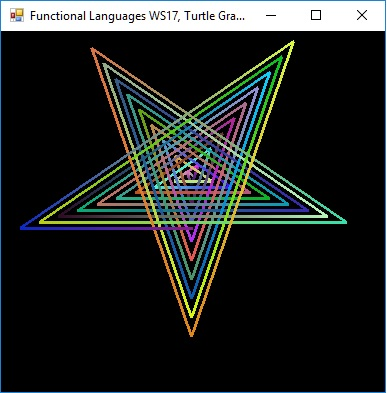
\includegraphics[width=0.5\textwidth]{star.jpg} %[bb=0 0 397 383]
	\caption{Turtle graphics for our star example program}
	\label{fig1}
\end{figure}

\begin{verbatim}
[
    Declare("count",0.0)
    Declare("starAngle",144.0)
    Declare("one",1.0)
    Declare("scale",2.0)
    Declare("iterations",100.0)
    While("count",Comparison.Less,"iterations", [
            Assign("dist","count",Mul,"scale")
            Forward "dist"
            Right "starAngle"
            Assign("count","count",Add,"one")
        ]
    )
]
\end{verbatim}


\noindent Let's look at how to implement imperative commands.\\
\noindent 
To declare a variable, we want to store our variable name in the turtle's variable map, and associate it with its value. Example implementation:

\begin{verbatim}
let setVariable (s : TurtleState) (varName : Variable) (value : Value) : TurtleState =
    { s with variables = Map.add varName value s.variables }

\end{verbatim}


\noindent Next, we want to assign a new variable using a binary operation on two existing variables. We would do the following:
\begin{itemize}
\item get the values both variables from the turtle's variable map
\item interpret the operation as function
\item apply the function on both values
\item store the result in the turtle's variable map under new name
\end{itemize}

\bigskip

\noindent Finally, we implement a while loop consisting of a loop body and a loop condition. The loop body is a list of commands. First, we implement a helper function that interprets many commands at once. We use this function to interpret the loop body. Using this helper function, we can do the following:
\begin{itemize}
\item evaluate the loop condition
\item if the evaluation results to true, interpret the body. This gives an intermediate TurtleState
\item make a recursive call with this intermediate TurtleState and the same loop commad
\item repeat until loop condition evaluates to false 
\item (make sure the loop terminates eventually, for example when food runs out!)
\end{itemize}

The function signatures are given in the template (marked with "todo").

\bigskip

\section{Implementation}

\begin{itemize}
\item Implementation of food supply and animation (5 points).
\item Implementation of imperative turtle commands (7 points).
\end{itemize}

\section{Files to submit}

Submit your project till 09.01. as a zip file without .git and obj folders.

\bigskip

Happy coding.

%\bibliographystyle{unsrt}
\bibliographystyle{unsrt}
\bibliography{references}
%\bibliography{references}
\end{document}
